\documentclass[12pt,a4paper]{article}
\usepackage{fontspec}
\XeTeXlinebreaklocale "th"
\XeTeXlinebreakskip=0pt plus 1pt
\defaultfontfeatures{Ligatures=TeX}
\setmainfont[Path={fonts/TH Sarabun PSK V-1/TH Sarabun PSK V-1/},Extension=.ttf,UprightFont={*},BoldFont={* Bold},ItalicFont={* Italic},BoldItalicFont={* BoldItalic}]{THSarabun}
\setmonofont{Latin Modern Mono}
\usepackage{amsmath,amssymb,mathtools,graphicx,float,caption,xcolor,hyperref,fancyhdr}
\usepackage{geometry,booktabs,array,tabularx,longtable,tikz}
\usetikzlibrary{positioning,arrows.meta,shapes.geometric}
\geometry{margin=0.82in}\setlength{\headheight}{15pt}
\pagestyle{fancy}\fancyhf{}\lhead{IEEE 14-bus with controller: ET-FCSPS vs BO}\rhead{\thepage}
\hypersetup{colorlinks=true,linkcolor=blue!55!black,urlcolor=blue!55!black}
\renewcommand{\arraystretch}{1.15}\emergencystretch=2em\linespread{1.12}
\renewcommand{\abstractname}{บทคัดย่อ}\renewcommand{\contentsname}{สารบัญ}
\renewcommand{\figurename}{รูปที่}\renewcommand{\tablename}{ตารางที่}
\newcommand{\code}[1]{\texttt{\detokenize{#1}}}
\newcommand{\vect}[1]{\boldsymbol{#1}}
\newcommand{\fcs}{ET--FCSPS}
\title{\textbf{IEEE 14-bus with Controller}\\
\large การเปรียบเทียบ Legacy Selector, Event-Triggered Finite-Control-Set Predictive Supervisor และ Bayesian-Optimisation Replay\\[1mm]
\normalsize ผลจาก Production All-KCL Time-Domain Simulation ครบ 160 วินาที}
\author{In-house Power-flow Project}\date{4 สิงหาคม 2569}

\begin{document}\maketitle
\begin{center}
\fcolorbox{teal!65!black}{teal!4}{\begin{minipage}{0.92\textwidth}
\textbf{ข้อสรุปสำหรับนำเสนอ}\quad ทั้งสามวิธีผ่าน simulation ถึง 160.000 s และเลือก action เดียวกัน คือ IBR1--IBR4 เป็น GFM โดย IBR1 เป็นเจ้าของ reference หลัง SG trip ดังนั้น raw trajectory ทุก field ที่ตรวจเปรียบเทียบกันตรงกัน โดยมี maximum absolute difference เท่ากับศูนย์ ในระบบขนาด 4 IBR นี้ \fcs{} เหมาะกว่า BO ในเชิงวิธีใช้งาน เพราะตรวจ feasible candidates ครบทั้ง 8 ตัวโดยตรง ขณะที่ BO ใช้ budget 8 evaluations จึงไม่ได้ลดจำนวน prediction และไม่ทำให้ response ดีขึ้น
\end{minipage}}
\end{center}

\begin{abstract}
รายงานนี้ทดสอบ supervisory controller สำหรับการเลือกชุดโหมด GFL/GFM และเจ้าของ reference ในระบบ IEEE 14-bus ที่มี SG หนึ่งเครื่องและ IBR สี่ตัว โดยใช้ production all-KCL composite DAE, fixed-step implicit trapezoidal integration, physical mode-transfer map และ atomic event transaction ชุดเดียวกันทุกกรณี เปรียบเทียบสาม arm ได้แก่ legacy selector จาก cache ที่ตรวจ provenance แล้ว, \fcs{} แบบ exhaustive และ BO แบบ finite-set offline replay ทุก arm ใช้ initial state, event chronology, post-trip dispatch, nonlinear equations, solver, tolerance และ time step $0.0125$ s เดียวกัน ผลคือทั้งสาม arm เลือก IBR ทั้งสี่เป็น GFM และกลับเป็น GFL หลัง SG handback ที่ $147.175$ s จึงให้ response เหมือนกันทุก field ข้อแตกต่างอยู่ที่กระบวนการค้นหา ไม่ใช่ dynamics รายงานนี้ไม่อ้าง deployment readiness เพราะ reserve ใช้ case-defined nameplate proxy และ BO ยังเป็น offline replay
\end{abstract}
\tableofcontents\newpage

\section{คำถามที่ต้องตอบจาก feedback}
\begin{enumerate}
\item IBR อยู่โหมดใดและเวลาใด: อ่านจาก committed hybrid-state timeline โดยตรง ไม่อนุมานจากสีกราฟหรือค่า index
\item ใคร form reference หลัง SG trip: ตัวที่ถูกเลือกเป็น \emph{reference owner} แยกจากจำนวน GFM ในรอบนี้ owner คือ IBR1 (device index 2, bus 2)
\item ใช้เกณฑ์อะไรสลับ: AGSI++/authenticated event ทำหน้าที่ trigger เท่านั้น ส่วน controller เลือก action จาก full-network voltage, frequency, RoCoF, current, active/reactive reserve, KCL, transition burden และ handback metric
\item สลับพร้อมกันหรือไม่: transaction ที่ 20 s commit IBR ทั้งสี่พร้อมกันใน accepted right limit เพราะ controller เลือก candidate เดียวกันทั้งชุด ไม่ใช่เพราะ local AGSI++ ชน threshold พร้อมกันโดยบังเอิญ
\item กลับสภาวะปกติอย่างไร: SG reclose ผ่าน synchronism guard ที่ 147.175 s แล้ว coordinated SG-reference handback คืน IBR1--IBR4 เป็น GFL แบบ atomic transaction
\end{enumerate}

\section{ขอบเขตและความยุติธรรมของการเปรียบเทียบ}
\begin{table}[H]\centering\caption{สิ่งที่ตรึงเหมือนกันทั้งสาม arm}
\begin{tabularx}{\textwidth}{p{.26\textwidth}X}\toprule
รายการ & สัญญาที่ใช้ \\\midrule
ระบบและ initial condition & IEEE 14-bus, 1 SG + 4 dual-mode IBR, accepted mixed-resource equilibrium เดียวกัน\\
เวลาและ solver & $0\le t\le160$ s, $\Delta t=0.0125$ s, full-KCL implicit trapezoidal step และ Newton contract เดียวกัน\\
เหตุการณ์ & SG trip 20 s; load $+20\%$ ที่ 50 s; bus-9 fault 85--85.15 s; line 6--13 trip 110 s; restore/reclose request 145 s\\
ค่าที่ห้ามเปลี่ยน & สมการ SG/IBR, threshold, dwell, dispatch, synchronizer, governor, protection gate, tolerance และ event order\\
สิ่งเดียวที่ controller เลือก & mode vector ของ IBR1--IBR4 และ GFM reference owner ณ SG-trip transaction\\
หลักฐาน & raw accepted production states เท่านั้น ไม่มี noise, smoothing, clipping หรือ display overlay ใน controller และตารางผล\\
\bottomrule\end{tabularx}\end{table}

Legacy arm ในรายงานนี้หมายถึง ``ไม่มี predictive controller'' แต่ยังมี authenticated legacy selector ที่จำเป็นต่อการเลือก voltage-forming source หลัง SG trip การปิด switching firmware ทั้งหมดจะทำให้ระบบไม่มี voltage-forming source และต้อง fail closed จึงไม่ใช่ comparator ที่มีความหมายทางกายภาพสำหรับ chronology นี้

\section{แบบจำลอง state ที่ controller ครอบอยู่}
Controller ไม่แก้สมการอุปกรณ์ แต่เลือก discrete mode ที่ครอบ continuous DAE เดิม
\begin{equation}
\vect{x}_{SG}=[\delta,\Delta\omega,E'_q,E'_d,E''_q,E''_d]^T,
\end{equation}
\begin{align}
\dot\delta&=\omega_0\Delta\omega,\\
2H\dot{\Delta\omega}&=P_m-P_e-D\Delta\omega,\\
T'_{d0}\dot E'_q&=E_{fd}+c_dE''_q-d_dE'_q,\\
T'_{q0}\dot E'_d&=c_qE''_d-d_qE'_d,\\
T''_{d0}\dot E''_q&=E'_q-E''_q-(X'_d-X''_d)I_d,\\
T''_{q0}\dot E''_d&=E'_d-E''_d+(X'_q-X''_q)I_q.
\end{align}
IBR แต่ละตัวใช้ dual-mode superset ที่มี GFM 13 states และ GFL 7 states
\begin{align}
\vect{x}_{GFM}&=[\delta_m,\delta_{IT},x_{wash},x_{Eint},\delta_{PLL},x_{PLL},I_{mv,f},I_{d,f},Q_{inv,f},V_{inv,f},I_{q,f},\delta_{IT,max},\delta_{IT,min}]^T,\\
\vect{x}_{GFL}&=[V_{t,f},P_f,I_{q,cmd,f},P_{ord},V_{LVPL,f},I_{p,reg},I_{q,reg}]^T.
\end{align}
Mode transfer ใช้ device-owned mapping จาก accepted left state แล้วแก้ algebraic right limit ใหม่ ไม่มีการ reset state เพื่อให้กราฟสวยขึ้น

\section{นิยาม AGSI++ และบทบาทที่ถูกต้อง}
AGSI++ เป็น local event indicator ที่ bounded ใน $[0,1]$ ไม่ใช่ผู้เลือก mode combination โดยตรง
\begin{align}
J_V&=\frac{|V-V_{ref}|}{0.10},&J_f&=\frac{|f-60|}{0.50},&J_R&=\frac{|df/dt|}{1.0},\\
J_P&=\frac{|P_{ref}-P|}{0.20},&J_{SCR}&=\max\left(0,\frac{3}{SCR}-1\right),&J_{lock}&=\frac{|v_q|}{0.10}.
\end{align}
ร่วมกับ $J_{GRA}=1-GRA$ แล้ว
\begin{equation}
AGSI^{++}=\min\!\left(1,\max\!\left(0,\frac{J_V+J_f+J_R+J_P+J_{SCR}+J_{lock}+J_{GRA}}{7}\right)\right).
\end{equation}
ความหมายตัวแปรคือ $V$ แรงดัน PCC, $V_{ref}$ ค่าอ้างอิง, $f$ ความถี่, $df/dt$ RoCoF, $P$ active power, $P_{ref}$ คำสั่ง active power, $SCR$ short-circuit ratio, $v_q$ q-axis voltage และ $GRA$ สถานะว่ามี grid-reference authority หรือไม่

\section{กลไกของ ET-FCSPS}
เมื่อ authenticated SG-trip event มาถึง controller สร้าง candidate จากทุก mode vector และทุก reference owner ที่เป็นไปได้ สำหรับ 4 IBR มี 32 mode-owner pairs แต่มี 8 pairs ที่ผ่าน authenticated selector/equilibrium/SSSA evidence
\begin{center}
\begin{tikzpicture}[node distance=9mm and 12mm,>=Stealth,every node/.style={font=\small},box/.style={draw,rounded corners,align=center,minimum width=32mm,minimum height=9mm},gate/.style={draw,diamond,aspect=2,align=center}]
\node[box] (a){accepted event-left state\\+ authenticated trigger};
\node[box,right=of a] (b){enumerate mode/owner\\candidate set};
\node[gate,right=of b] (c){hard screen\\ผ่านหรือไม่};
\node[box,below=of c] (d){0.25-s nonlinear\\full-KCL prediction};
\node[box,left=of d] (e){คำนวณ cost\\และ deterministic rank};
\node[box,left=of e] (f){stale-snapshot guard\\+ atomic commit};
\draw[->](a)--(b);\draw[->](b)--(c);\draw[->](c)--node[right]{ผ่าน}(d);\draw[->](d)--(e);\draw[->](e)--(f);
\draw[->,red!70!black](c.east)--++(12mm,0)|-node[pos=.25,right]{ไม่ผ่าน: reject}(f.south);
\end{tikzpicture}
\end{center}
ทุก prediction เริ่มจาก accepted event-left state fingerprint เดียวกัน ผ่าน SG breaker transition, physical mode transfer, post-trip dispatch และ full-KCL right-limit solve เดียวกัน จากนั้นใช้ production trapezoidal kernel ครบ horizon $T_p=0.25$ s

Hard constraints ตรวจ KCL, $V_{min}\le|V|\le V_{max}$, current limit, frequency, RoCoF, reserve availability, online/reference capability, dwell และ lockout ก่อน cost ส่วน cost คือ
\begin{equation}
J=\sum_{k}w_k\phi_k,
\end{equation}
โดย $\phi_k$ ครอบคลุม voltage, frequency, RoCoF, reserve $P/Q$, current utilization, handback mismatch, จำนวน GFM และจำนวน switch น้ำหนักถูก freeze ก่อนดูผล

\section{BO comparator ทำงานอย่างไร}
BO ใช้ feature ของ candidate mode-owner, RBF Gaussian-process surrogate และ Expected Improvement
\begin{align}
k(\vect{z},\vect{z}')&=\exp\!\left[-\frac{\|\vect{z}-\vect{z}'\|^2}{2\ell^2}\right],\\
EI(\vect{z})&=(J_{best}-\mu)\Phi(\zeta)+\sigma\phi(\zeta),\qquad
\zeta=\frac{J_{best}-\mu}{\sigma}.
\end{align}
Comparator นี้เป็น \textbf{offline finite-set replay}: รับ immutable trial table เดียวกับ ET แล้วเปิดเผย cost ตามลำดับ BO ไม่เรียก Optimization Toolbox และไม่แก้ production states ระหว่างค้นหา Budget ถูก freeze ที่ 8 evaluations

\section{ผล simulation 160 วินาที}
\begin{table}[H]\centering\caption{ผล raw production ของสาม arm}
\small\begin{tabular}{lrrr}\toprule
ตัวชี้วัด & Legacy & ET-FCSPS & BO replay\\\midrule
ปลายทางเวลา (s) & 160.000 & 160.000 & 160.000\\
$\min |V|$ รวม fault (pu) & 0.060077 & 0.060077 & 0.060077\\
$\max |V|$ (pu) & 1.133568 & 1.133568 & 1.133568\\
ช่วงความถี่ online (Hz) & 58.3238--63.5606 & 58.3238--63.5606 & 58.3238--63.5606\\
maximum current utilization & 1.0000 & 1.0000 & 1.0000\\
จำนวน mode switches รวม & 8 & 8 & 8\\
aggregate GFM-on time (s) & 508.700 & 508.700 & 508.700\\
SG reclose/handback (s) & 147.175 & 147.175 & 147.175\\
max accepted residual & $9.982\times10^{-9}$ & $9.982\times10^{-9}$ & $9.982\times10^{-9}$\\
prediction evaluations & -- & 8 & 8\\
selected GFM & IBR1--IBR4 & IBR1--IBR4 & IBR1--IBR4\\
\bottomrule\end{tabular}\end{table}

\begin{figure}[H]\centering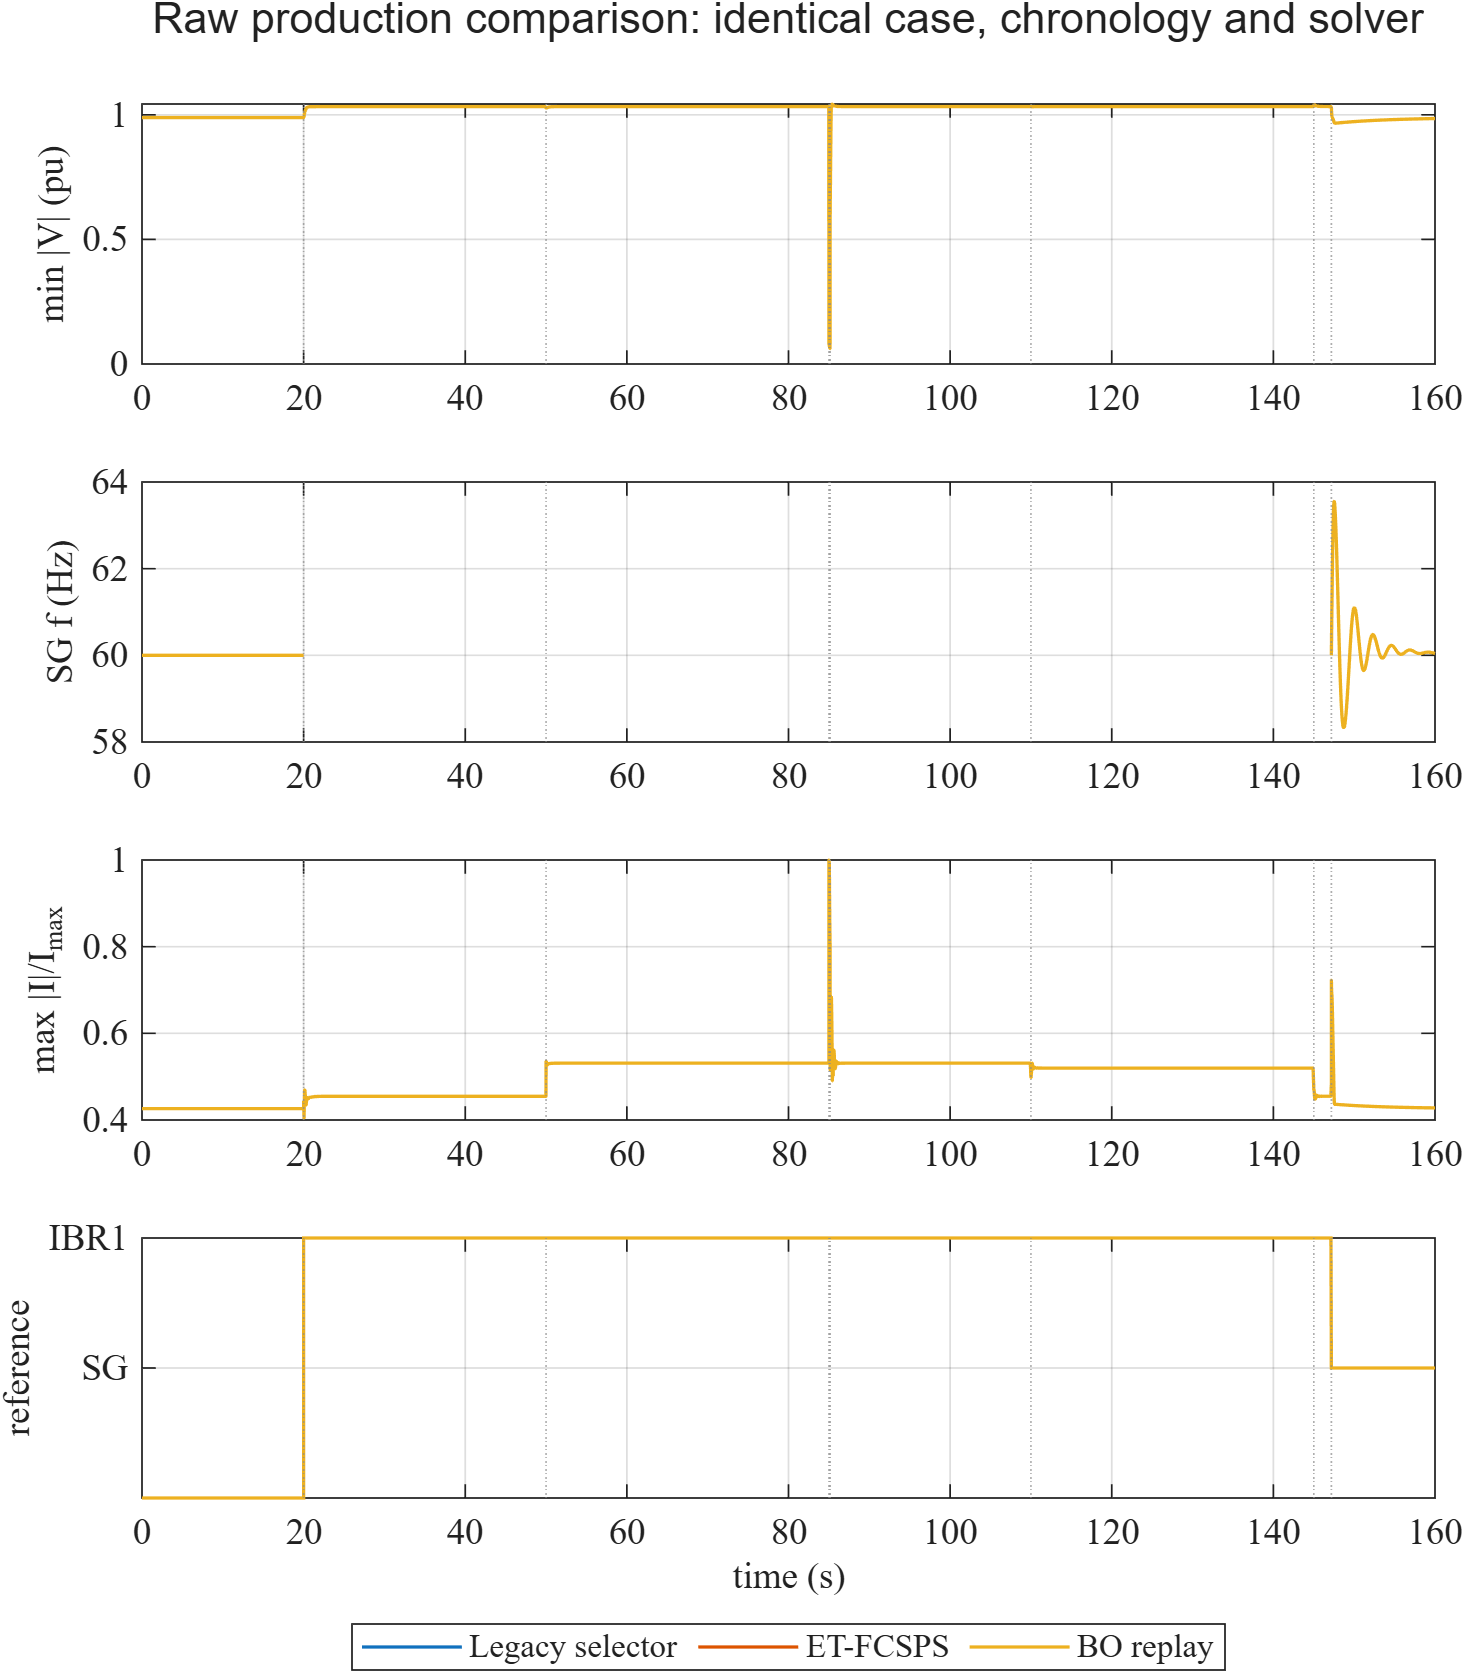
\includegraphics[width=6.4in]{figures/ieee14_controller_compare/controller_comparison_system.png}
\caption{เปรียบเทียบ raw system response เส้นทั้งสามทับกันพอดีเพราะเลือก action เดียวกัน ไม่ใช่การ smoothing หรือ copy trajectory}\end{figure}
\begin{figure}[H]\centering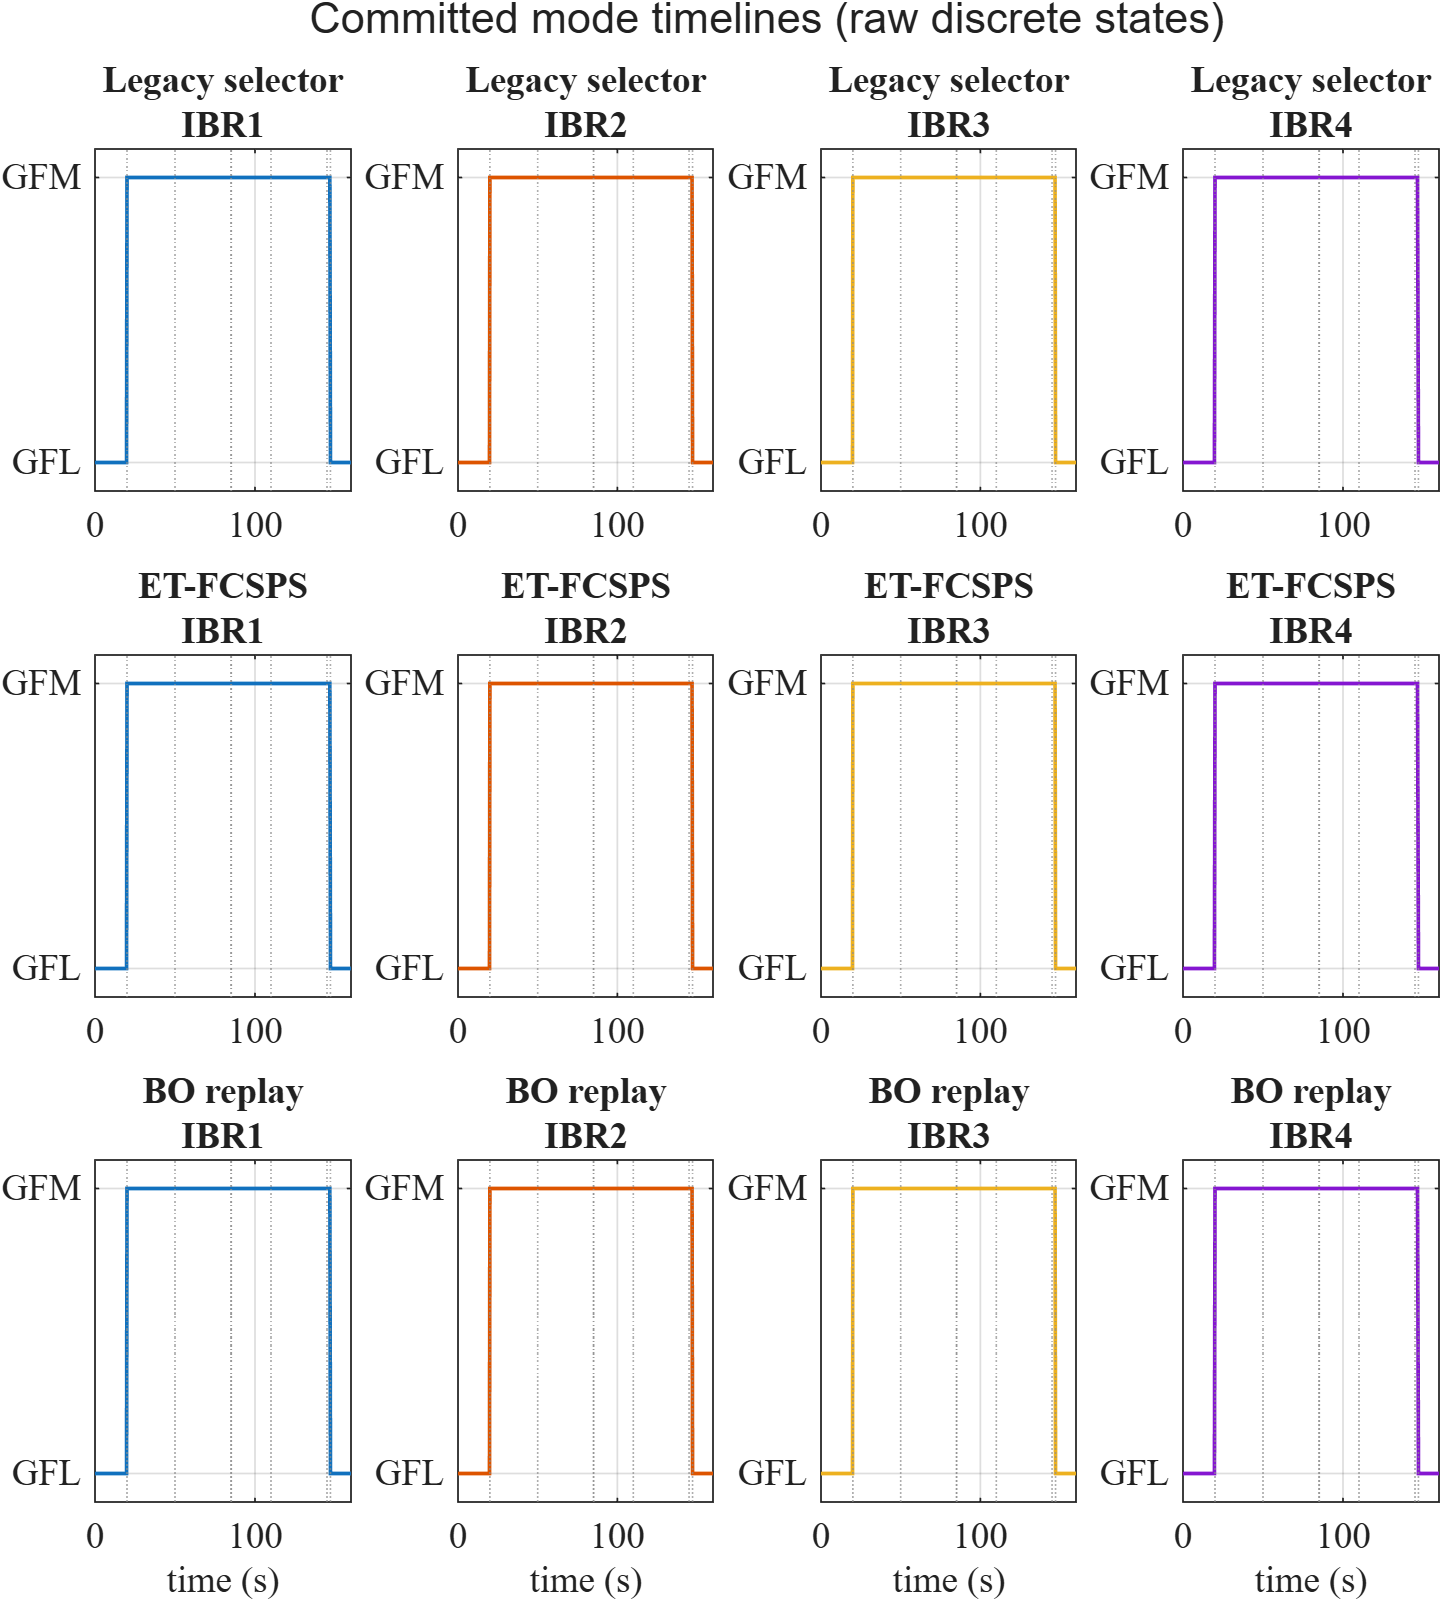
\includegraphics[width=6.4in]{figures/ieee14_controller_compare/controller_comparison_modes.png}
\caption{Committed mode timeline: IBR1--IBR4 เปลี่ยน GFL$\rightarrow$GFM ที่ 20 s และกลับ GFM$\rightarrow$GFL หลัง coordinated handback}\end{figure}
\begin{figure}[H]\centering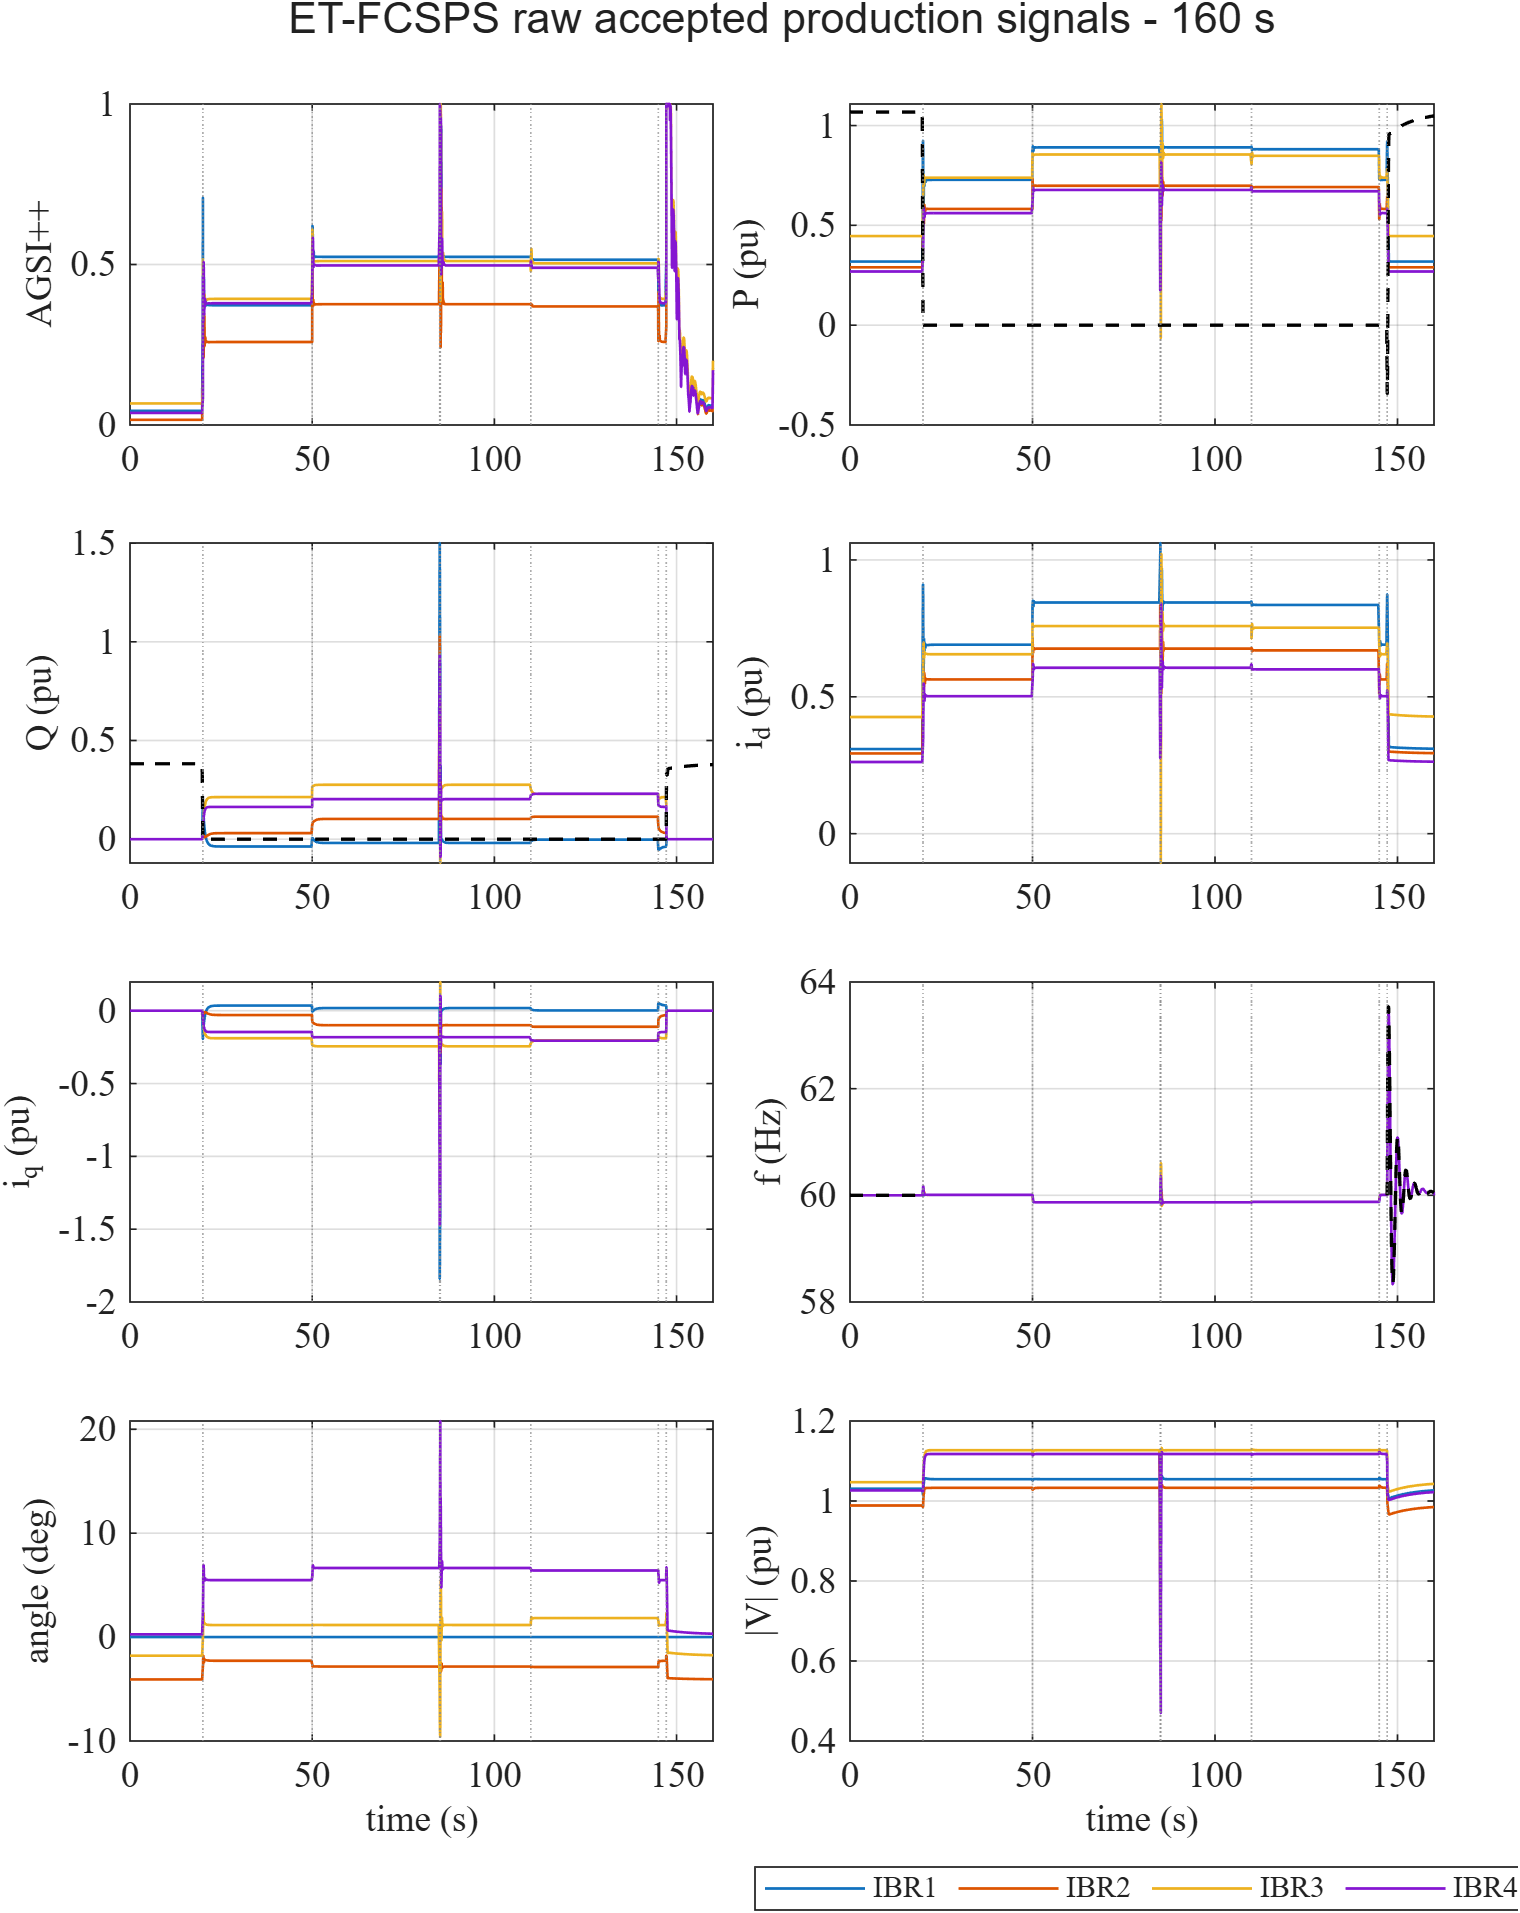
\includegraphics[width=6.4in]{figures/ieee14_controller_compare/controller_et_fcsps_raw_response.png}
\caption{Raw ET-FCSPS signals ครบ AGSI++, $P,Q,i_d,i_q,f$, angle และ voltage; เส้นดำประใน $P,Q,f$ คือ SG}\end{figure}
\begin{figure}[H]\centering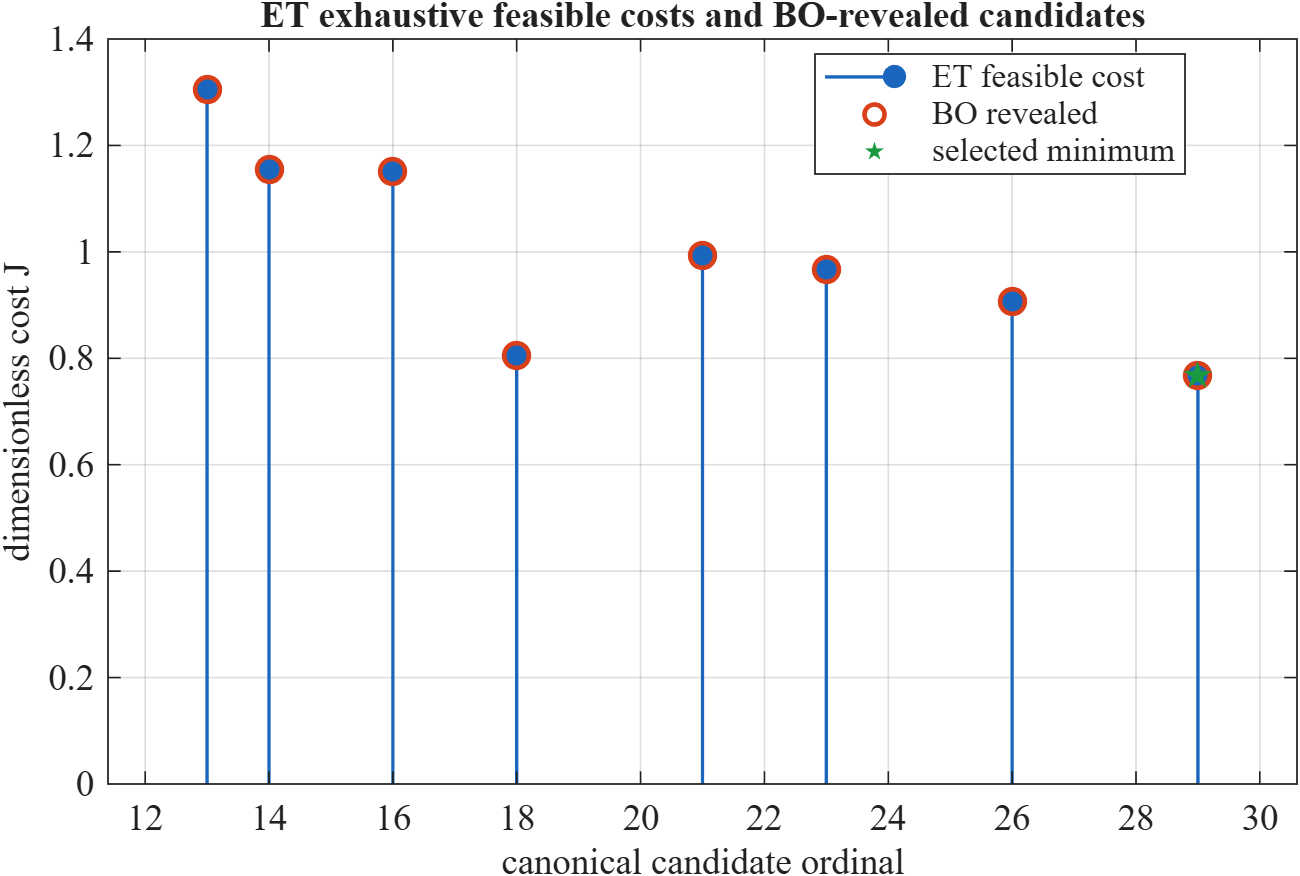
\includegraphics[width=6.4in]{figures/ieee14_controller_compare/controller_candidate_costs.png}
\caption{Cost ของ feasible candidates ทั้ง 8 ตัว วงกลมสีส้มแสดงว่าด้วย budget 8 BO ต้องเปิดเผยครบทุกตัว จึงไม่มี evaluation saving}\end{figure}

\section{ทำไมผลทั้งสามเหมือนกัน และวิธีใดดีกว่า}
Maximum absolute difference ระหว่าง raw arrays ของทั้งสาม arm เท่ากับศูนย์ใน AGSI++, mode, $P,Q,i_d,i_q,f$, angle, voltage, minimum network voltage, reference code และ SG traces สาเหตุคือ candidate ที่มี GFM ครบสี่ตัวและ IBR1 เป็น owner มี cost ต่ำสุดและเป็น legacy choice อยู่แล้ว เมื่อ discrete action และ continuous initial state หลัง transaction เหมือนกัน deterministic production solver จึงให้ trajectory เดียวกัน

สำหรับ case นี้ \textbf{ET-FCSPS เป็นตัวเลือกที่เหมาะกว่า BO} ด้วยเหตุผลสามข้อ: (1) feasible universe มีเพียง 8 ตัว จึง exhaustive ได้ตรง ๆ (2) BO budget เท่ากับ 8 จึงไม่ลด nonlinear evaluations และ (3) ET มี deterministic global minimum บน finite set โดยไม่เพิ่ม surrogate hyperparameter อย่างไรก็ตาม BO อาจมีประโยชน์เมื่อจำนวน IBR มากจน candidate universe โตแบบ exponential แต่ต้องทดสอบด้วย budget ที่น้อยกว่า feasible count และวัด regret จริงก่อนสรุป

Wall time ของ ET และ BO long runs เท่ากับ 2182.918 s และ 2223.825 s ตามลำดับ ความต่างประมาณ 1.9\% ไม่ควรตีความเป็นข้อได้เปรียบของ controller เพราะทั้งสองใช้ trajectory เดียวกันและ candidate evidence ถูกสร้างร่วมกัน ส่วน runtime ของ legacy มาจาก cache คนละรอบและไม่ใช้เป็น speed benchmark

\section{ข้อจำกัดและสิ่งที่ยังไม่ควรอ้าง}
\begin{itemize}
\item BO เป็น offline replay ไม่ใช่ online BO authority และในรอบนี้ไม่ได้ประหยัด evaluation
\item P/Q reserve ใช้ case-defined nameplate proxy ไม่ได้พิสูจน์ energy duration, storage SOC หรือ hardware reserve
\item ผลนี้พิสูจน์ software/controller behavior ใน chronology เดียว ไม่ใช่ protection, HIL หรือ field readiness
\item การกลับปกติหมายถึง topology/reference/mode/voltage transaction สำเร็จและระบบ settle ใกล้ 60 Hz ไม่ใช่การพิสูจน์ secondary-frequency restoration สำหรับทุก operating condition
\item ไม่ได้ปรับ threshold, weight, equation หรือ solver หลังเห็นผล และไม่ได้ใส่ noise ใน raw evidence
\end{itemize}

\section{การทำซ้ำ}
\begin{verbatim}
pf_init_paths;
addpath(fullfile('scripts','reporting'));
out = run_ieee14_controller_comparison(reuse_completed=true);
generate_ieee14_controller_comparison_figures;
\end{verbatim}
หลักฐานหลักอยู่ที่ \code{output/diagnostics/ieee14_controller_compare/} และรูปอยู่ที่ \code{docs/source/figures/ieee14_controller_compare/}
\end{document}
